\section{Actividad 3}

\subsection*{Se tiene la función de densidad de la Fig.~\ref{fig:diagrama_3}}

\begin{figure}[H]
    \centering
    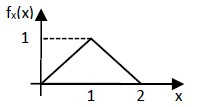
\includegraphics[width=0.35\linewidth]{imagenes/Actividad_3/actividad_3.jpg}
    \caption{Función de densidad triangular.}
    \label{fig:diagrama_3}
\end{figure}

La función de densidad se describe analíticamente como:
\[
f_X(x)=
\begin{cases}
x, & 0 \leq x \leq 1, \\[6pt]
2-x, & 1 < x \leq 2, \\[6pt]
0, & \text{otro caso}.
\end{cases}
\]

%---------------------------------------------------------
\subsection*{a) Cálculo analítico de la media, varianza y desviación estándar}

La media se obtiene como:
\[
\mu = E[X] = \int_0^1 x \cdot x \,dx + \int_1^2 x (2-x)\,dx = 1.
\]

La varianza se obtiene mediante:
\[
\sigma^2 = E[(X-\mu)^2] = \frac{1}{6} \approx 0.1667,
\]
y por lo tanto,
\[
\sigma = \sqrt{\sigma^2} \approx 0.4082.
\]

%---------------------------------------------------------
\subsection*{b) Función de distribución acumulada}

Integrando por tramos la densidad, se obtiene:
\[
F_X(x)=
\begin{cases}
0, & x \leq 0, \\[6pt]
\dfrac{x^2}{2}, & 0 < x \leq 1, \\[10pt]
-\dfrac{x^2}{2}+2x-1, & 1 < x \leq 2, \\[6pt]
1, & x > 2.
\end{cases}
\]

\begin{figure}[H]
    \centering
    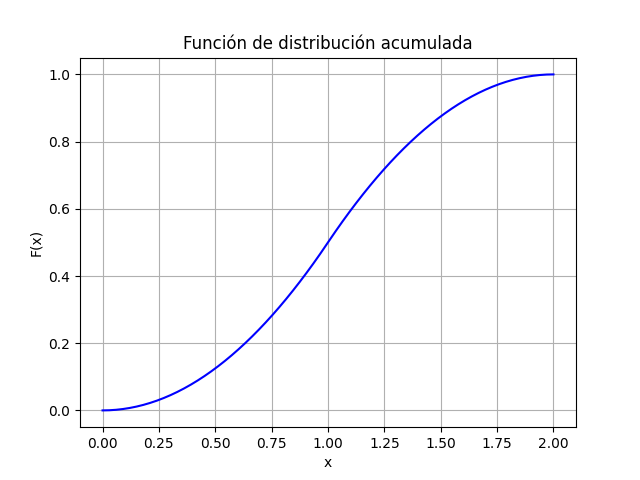
\includegraphics[width=0.6\linewidth]{imagenes/Actividad_3/cdf.png}
    \caption{Función de distribución acumulada \(F_X(x)\).}
    \label{fig:cdf}
\end{figure}

%---------------------------------------------------------
\subsection*{c) Cálculo de la probabilidad \( P(0.75 \leq X \leq 1.75) \)}

\[
P(0.75 \leq X \leq 1.75) = F_X(1.75) - F_X(0.75).
\]

Evaluando:
\[
F_X(0.75) = \frac{0.75^2}{2} = 0.28125,
\qquad
F_X(1.75) = -\frac{1.75^2}{2} + 2(1.75) - 1 = 0.96875.
\]

Por lo tanto:
\[
P(0.75 \leq X \leq 1.75) = 0.96875 - 0.28125 = 0.6875.
\]

%---------------------------------------------------------
\subsection*{d) Generación de muestras y graficación}

Se generaron 500 muestras aleatorias a partir de la distribución, usando el método de la transformada inversa.  
En la Fig.~\ref{fig:histograma} se muestra el histograma obtenido, donde se aprecia la forma triangular característica de la densidad.

\begin{figure}[H]
    \centering
    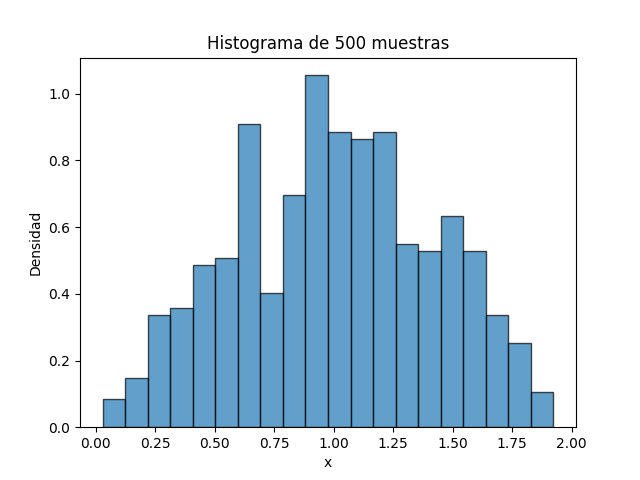
\includegraphics[width=0.6\linewidth]{imagenes/Actividad_3/histograma.png}
    \caption{Histograma de 500 muestras generadas a partir de la densidad.}
    \label{fig:histograma}
\end{figure}

La media empírica se calcula a partir de las muestras como:
\[
\bar{X} = \frac{1}{n}\sum_{i=1}^{n} x_i,
\]
y la varianza empírica mediante:
\[
s^2 = \frac{1}{n}\sum_{i=1}^{n} (x_i - \bar{X})^2.
\]

Al evaluar estas expresiones con las 500 muestras generadas, se obtienen valores numéricos que se aproximan a los resultados teóricos:
\[
\mu = 1, \qquad \sigma^2 = \tfrac{1}{6}.
\]


